\documentclass[12pt,a4paper]{article}
\usepackage[utf8]{inputenc}
\usepackage{amsmath}
\usepackage{amsfonts}
\usepackage{amssymb}
\usepackage{float}
\usepackage{csvsimple}
\usepackage{enumerate}
\usepackage{hyperref}
\usepackage{graphicx}
\usepackage{gensymb}
\usepackage{txfonts}
\usepackage{listings}
\usepackage{cleveref}
\usepackage{xcolor}
\parindent 0px
\usepackage[none]{hyphenat}
\usepackage{listings} %Package for the enviroment in which we write code 
\usepackage[left=1cm,right=1cm,top=2cm]{geometry}
\pagenumbering{arabic}
%Some custom colours
\definecolor{codegreen}{rgb}{0,0.6,0}
\definecolor{codegray}{rgb}{0.5,0.5,0.5}
\definecolor{codepurple}{rgb}{0.58,0,0.82}
\definecolor{backgroundcolour}{rgb}{0.95,0.95,0.92}

%Shortcut for strings "Code" and "List of Code"
\renewcommand{\lstlistingname}{Code}
\renewcommand{\lstlistlistingname}{List of Code}

%This is the template for code styling, named as "mystyle"
\lstdefinestyle{mystyle}{
	backgroundcolor=\color{backgroundcolour},
	basicstyle=\ttfamily\small,
	commentstyle=\color{green!60!black},
	keywordstyle=\color{magenta},
	stringstyle=\color{blue!50!red},
	showstringspaces=false, 
	captionpos=b, 
	tabsize=2,
	frame=single,
	breaklines=true,
	inputpath=code
}  

%%%%%%%%%%%%%%%%%%%%%%%%%%%%%%%%%%%%%%%%%%%%%%%%%%%%%%%%%%%%%%%%%%%%%%%%%%%%%%%%%%%%%%%%%%%%%%%%%%%%%%%%%%%%%%%%
\title{Database Implementation}
\author{ Bommineni Vishwajith Reddy \\ EE21BTECH11012 }
\date{}

\begin{document}
	\maketitle
	
	\tableofcontents
	\newpage
	
	\section{ER-Diagram}
		\begin{figure}[H]
		\centering
		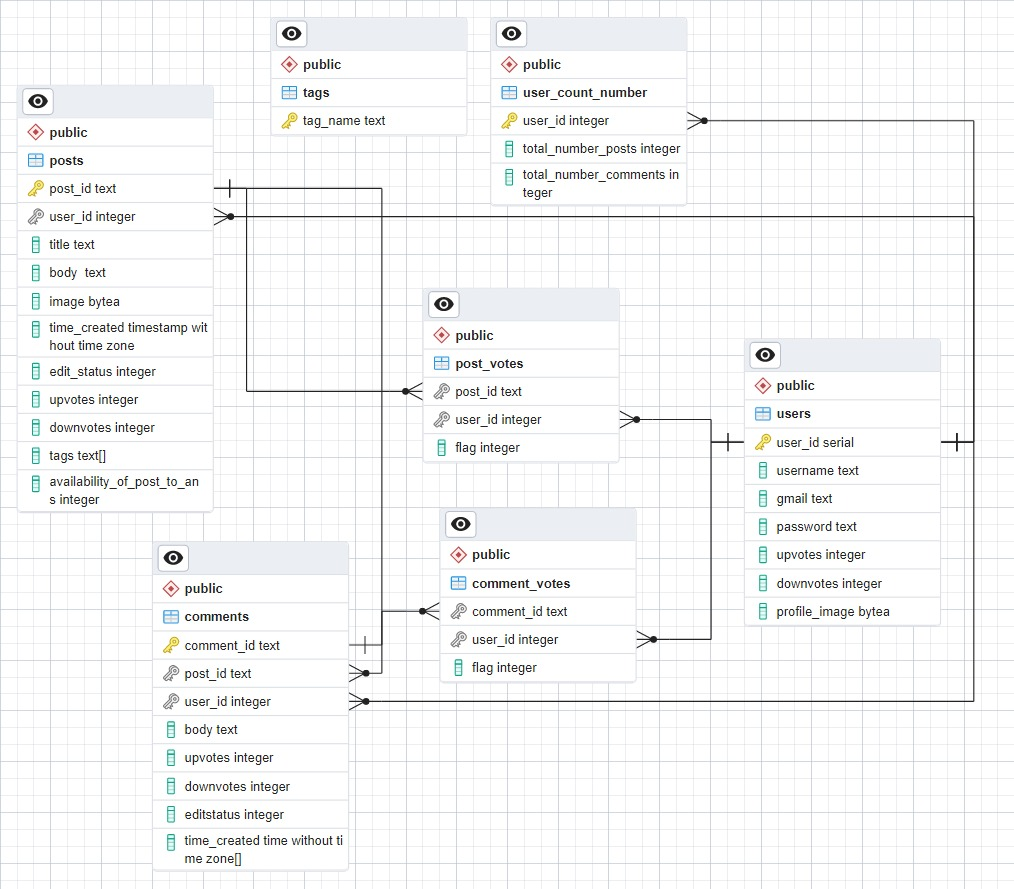
\includegraphics[width=1\textwidth]{ER_dig}
		\caption{ERD figure}
	\end{figure}
\newpage
	\section{Relations}
	\begin{itemize}
		\item   The DDL of the database can be found in the file \textbf{ddl.sql}
	\end{itemize}
	\subsection{users}
	\subsubsection{Usage}
		\begin{itemize}
		\item This table stores the information of users
	\end{itemize}
\subsubsection{Attributes}
	\begin{itemize}
		\item \textbf{user\_id: }This is auto generated user identification number.
		\item \textbf{username: }Attribute which stores the username of the user.
		\item \textbf{gmail: }Attribute which stores the e-mail of the user.
		\item \textbf{password: }Attribute which stores the password of the user with \textbf{MD5} hashing.
		\item \textbf{upvotes: }Attribute which stores the total upvotes count of the user.
		\item \textbf{downvotes: }Attribute which stores the total downvotes count of the user.
		\item \textbf{profile\_image: }Attribute which stores the profile picture of the user.
	\end{itemize}
	\subsection{posts}
		\subsubsection{Usage}
	\begin{itemize}
		\item This table stores the information regarding posts 
	\end{itemize}
	\subsubsection{Attributes}
	\begin{itemize}
		\item \textbf{post\_id: }This is auto generated post identification string.
		\item \textbf{user\_id: }Stores the user\_id of the user who made the post.
		\item \textbf{title: }Attribute which stores the title of the post.
		\item \textbf{body:} Attribute which stores the body of the post.
		\item \textbf{image: }Attribute which stores the image corresponding to post.
		\item \textbf{time\_created: }Attribute which stores the information of time of creation of post.
		\item \textbf{edit\_status: }Attribute which stores the info regarding if the post is edited or not.
		\item \textbf{upvotes: }Attribute which stores the upvotes count for the post.
		\item \textbf{downvotes: }Attribute which stores the downvotes count for the post.
		\item \textbf{tag: }Attribute which stores the information regarding tags assigned to the post.
		\item \textbf{availability\_of\_post\_to\_ans: }Attribute which stores the information regarding if the post is still open for answering.
	\end{itemize}
	\subsection{comments}
		\subsubsection{Usage}
\begin{itemize}
	\item This table stores the information regarding comments 
\end{itemize}
\subsubsection{Attributes}
\begin{itemize}
	\item \textbf{comment\_id: }This is auto generated comment identification string.
	\item \textbf{post\_id: }Stores the post\_id for which post the current comment belongs to.
	\item \textbf{user\_id: }Stores the user\_id of the user who made the post.
	\item \textbf{body:} Attribute which stores the body of the comment.
	\item \textbf{upvotes: }Attribute which stores the upvotes count for the comment.
	\item \textbf{downvotes: }Attribute which stores the downvotes count for the comment.
	\item \textbf{edit\_status: }Attribute which stores the info regarding if the comment is edited or not.
	\item \textbf{time\_created: }Attribute which stores the information of time of creation of comment.
\end{itemize}
	\subsection{tags}
		\subsubsection{Usage}
\begin{itemize}
	\item This table stores the information regarding tags available in the website to choose for a question. 
\end{itemize}
\subsubsection{Attributes}
\begin{itemize}
	\item \textbf{tag\_name: }Attribute which stores tag name.
\end{itemize}

	\subsection{user\_count\_number}
		\subsubsection{Usage}
\begin{itemize}
	\item This table stores the information regarding activity of the user.
\end{itemize}
\subsubsection{Attributes}
\begin{itemize}
	\item \textbf{user\_id:} This is the user\_id of the user.
	\item \textbf{total\_number\_posts:} This is the count of total number of posts made by the user.
	\item \textbf{total\_number\_comments:} This is the count of total comments made by the user.
\end{itemize}

	\subsection{post\_votes}
		\subsubsection{Usage}
\begin{itemize}
	\item This table stores the information regarding which user upvoted/ downvoted a post.
\end{itemize}
\subsubsection{Attributes}
\begin{itemize}
	\item \textbf{post\_id:} This is the post\_id of the post.
	\item \textbf{user\_id:} This is the user\_id of person who upvotes or downvoted the post.
	\item \textbf{flag:} Status of the post w.r.t the user with id post\_id whether it is upvoted/ downvoted/ no action.
\end{itemize}

	\subsection{comment\_votes}	
		\subsubsection{Usage}
\begin{itemize}
	\item This table stores the information regarding which user upvoted/ downvoted a comment.
\end{itemize}
\subsubsection{Attributes}
\begin{itemize}
	\item \textbf{post\_id:} This is the comment\_id of the comment.
	\item \textbf{user\_id:} This is the user\_id of person who upvotes or downvoted the comment.
	\item \textbf{flag:} Status of the post w.r.t the user with id comment\_id whether it is upvoted/ downvoted/ no action.
\end{itemize}



	\section{Functions}
	\begin{itemize}
	\item For details regarding functions used in the database, look into the file  \textbf{functions.sql}
\end{itemize}
	
	\begin{lstlisting}[language=SQL, style = mystyle]
		login(user_id_in TEXT, pass TEXT)
	\end{lstlisting}
\begin{itemize}
	\item The above function \textbf{login()}, takes in two arguments \textbf{user\_id} and \textbf{password} for the account and returns:
	\begin{itemize}
		\item $1$ if given credentials are correct
		\item $0$ if given credentials are incorrect
	\end{itemize}
\item This function is called when a user tries to login.
\end{itemize}
	\begin{lstlisting}[language=SQL, style = mystyle]
	votes_track_post(user_idi int, post_idi TEXT, votess int)
\end{lstlisting}
\begin{itemize}
	\item The above function \textbf{votes\_track\_post()}, takes in three arguments \textbf{user\_id}, \textbf{post\_id} and \textbf{votess} (+1 for upvote, -1 for downvote) for the account and returns:
	\begin{itemize}
		\item $1$ if task is successful
		\item $0$ if task is unsuccessful
	\end{itemize}
\item This function is called when a user upvotes/ downvotes a post.
\end{itemize}
	
	\begin{lstlisting}[language=SQL, style = mystyle]
	votes_track_comment(user_idi int, comment_idi TEXT, votess int)
\end{lstlisting}
\begin{itemize}
	\item The above function \textbf{votes\_track\_comment()}, takes in three arguments \textbf{user\_id}, \textbf{comment\_id} and \textbf{votess} (+1 for upvote, -1 for downvote) for the account and returns:
	\begin{itemize}
		\item $1$ if task is successful
		\item $0$ if task is unsuccessful
	\end{itemize}
	\item This function is called when a user upvotes/ downvotes a comment.
\end{itemize}
	
		\begin{lstlisting}[language=SQL, style = mystyle]
update_password(user_id_in int , pass text)
	\end{lstlisting}
	\begin{itemize}
		\item The above function \textbf{update\_password()}, takes in two arguments \textbf{user\_id}, \textbf{password} and returns:
		\begin{itemize}
			\item $1$ if task is successful
			\item $0$ if task is unsuccessful
		\end{itemize}
		\item This function is called when a user tries to change the account's password. 
	\end{itemize}

		\begin{lstlisting}[language=SQL, style = mystyle]
update_upvotes_downvotes_post(post_id_in text, up int, down int)
\end{lstlisting}
\begin{itemize}
	\item The above function \textbf{update\_upvotes\_downvotes\_post()}, takes in three arguments \textbf{post\_id}, \textbf{up} (default fixed value = +1), \textbf{down} (default fixed value = -1) and returns:
	\begin{itemize}
		\item $1$ if task is successful
		\item $0$ if task is unsuccessful
	\end{itemize}
	\item This function is called when a user's post is upvoted/ downvoted.
\end{itemize}

		\begin{lstlisting}[language=SQL, style = mystyle]
	update_upvotes_downvotes_comment(comment_id_in text, up int, down int)
\end{lstlisting}
\begin{itemize}
	\item The above function \textbf{update\_upvotes\_downvotes\_comment()}, takes in three arguments \textbf{comment\_id}, \textbf{up} (default fixed value = +1), \textbf{down} (default fixed value = -1) and returns:
	\begin{itemize}
		\item $1$ if task is successful
		\item $0$ if task is unsuccessful
	\end{itemize}
	\item This function is called when a user's comment is upvoted/ downvoted.
\end{itemize}

		\begin{lstlisting}[language=SQL, style = mystyle]
search_posts_by_user_id(user_id_in int)
\end{lstlisting}
\begin{itemize}
	\item The above function \textbf{search\_posts\_by\_user\_id()}, takes in one argument \textbf{user\_id} and returns:
	\begin{itemize}
		\item All the posts made by the user.
	\end{itemize}
	\item This function is called when a we need to know about the posts made by a user.
\end{itemize}

		\begin{lstlisting}[language=SQL, style = mystyle]
search_posts_by_tags(tags text[])
\end{lstlisting}
\begin{itemize}
	\item The above function \textbf{search\_posts\_by\_tags()}, takes in one argument \textbf{tags} (An array of tag names) and returns:
	\begin{itemize}
		\item All the posts which have tags as the given tags.
	\end{itemize}
	\item This function is called when a we need to know about the posts made by some specific tags.
\end{itemize}


	\section{Triggers}

	\subsection{Insert}
		\begin{itemize}
	\item For details regarding triggers used in the database, look into the file \textbf{insert\_triggers.sql}
			\begin{lstlisting}[language=SQL, style = mystyle]
		insert_users_1 
	\end{lstlisting}
\textbf{Trigger function: }insert\_users\_table\_1()\\
\textbf{Task: }Sets default password as username of the user before insertion of new user to \textbf{users} table.
			\begin{lstlisting}[language=SQL, style = mystyle]
	insert_users_2
\end{lstlisting}
\textbf{Trigger function: }insert\_users\_table\_2()\\
\textbf{Task: }Adds new tuple to \textbf{user\_count\_number} table after insertion of new tuple to \textbf{users} table.
			\begin{lstlisting}[language=SQL, style = mystyle]
	insert_posts 
\end{lstlisting}
\textbf{Trigger function: }insert\_posts\_table()\\
\textbf{Task: }Checks if given tags assigned to a post are valid or not and updates the user's count of post count by 1 if the post is  valid to be posted.
			\begin{lstlisting}[language=SQL, style = mystyle]
	insert_comments 
\end{lstlisting}
\textbf{Trigger function: }insert\_comments\_table()\\
\textbf{Task: }Assigns comment\_id for the comment and updates the user's count of comment count by 1.
\end{itemize}
	\subsection{Update}
		\begin{itemize}
	\item For details regarding triggers used in the database, look into the file \textbf{update\_triggers.sql}
				\begin{lstlisting}[language=SQL, style = mystyle]
		update_to_post 
	\end{lstlisting}
	\textbf{Trigger function: }update\_post()\\
	\textbf{Task: }This trigger is called when a post is edited, based on that flag value is set.
				\begin{lstlisting}[language=SQL, style = mystyle]
update_to_comment
\end{lstlisting}
\textbf{Trigger function: }update\_comment()\\
\textbf{Task: }This trigger is called when a comment is edited, based on that flag value is set.
	
\end{itemize}
	\subsection{Delete}
		\begin{itemize}
	\item For details regarding triggers used in the database, look into the file \textbf{delete\_triggers.sql}

					\begin{lstlisting}[language=SQL, style = mystyle]
	delete_comments_tab
	\end{lstlisting}
\textbf{Trigger function: }delete\_comments\_table()\\
\textbf{Task: }This trigger is called when a comment is deleted, this resets the total upvotes and downvotes of the user by deleting the contribution of deleted comment.
					\begin{lstlisting}[language=SQL, style = mystyle]
delete_posts_tab
\end{lstlisting}
\textbf{Trigger function: }delete\_posts\_table()\\
\textbf{Task: }This trigger is called when a post is deleted, this resets the total upvotes and downvotes of the user by deleting the contribution of deleted post.
	\item \textbf{Note: }Any deletions which are done on \textbf{users} table this is handled in other tables by using the \textbf{on delete cascade} foerign key constraint.
\end{itemize}
			

	\section{Data Filling}
	\begin{itemize}
		\item For filling data in the database, look into the file  \textbf{data\_filling.sql}
	\end{itemize}
\end{document}



